

%\documentclass{book}\begin{document}<content\end{document}
\documentclass[letter, 11pt, margins=0.25in]{texMemo}  % The texMemo package by Rob Oakes.

\usepackage{amsmath}
\usepackage{color, soul}
\usepackage{dcolumn}
    \newcolumntype{d}[1]{D{.}{.}{#1}}
\usepackage[colorlinks=true, citecolor=blue]{hyperref}
\usepackage{enumitem}
\usepackage{graphicx, lipsum}

\usepackage[LGRgreek]{mathastext}

\usepackage{matlab-prettifier}
\usepackage{multirow}

\usepackage{natbib}
\bibliographystyle{apalike}

\usepackage[table]{xcolor}
\definecolor{maroon}{cmyk}{0,0.87,0.68,0.32}
\definecolor{LightCyan}{rgb}{0.88,1,1}
\definecolor{Gray}{gray}{0.85}


\memodate{\today~(Submitted)}
\memosubject{ACS 547, Noise Control Applications - Module 2 Assignment\\}



\begin{document}

\maketitle


\vspace{-0.25cm}
\section*{Problem 1 - Modal Behaviour of a Cylindrical Room}

The Matlab code for this problem is listed in Appendix~\ref{appendix:problem1}.

\vspace{-0.25cm}
\subsection*{Problem 1a}

The lowest cut-on frequency for a rectangular duct with air flow is given by equation,

\vspace{-0.25cm}
\begin{equation}
    f_{cut-on} = 0.5 \cdot \frac{c}{L}
\end{equation}

where $c$ is the speed of sound in air, 343~$\frac{m}{s}$,  and $L$ is the largest side of the rectangular cross-section.

\vspace{0.25cm}
With cross-sectional dimensions of $L_x = 12~cm$ and $L_y = 20~cm$, the lowest cut-on frequency for this rectangular duct is,

\vspace{-0.25cm}
\begin{equation*}
    f_{cut-on} = 0.5 \cdot \frac{ 343~\frac{m}{s} }{ 0.20~m } = \boldsymbol{857.5~Hz}
\end{equation*}



\vspace{-0.25cm}
\subsection*{Problem 1b}

The lowest cut-on frequency for a circular duct with air flow with the same cross-sectional area as the rectangular duct in part (a.) can be calculated using equation,

\vspace{-0.25cm}
\begin{equation}
    f_{cut-on} = 0.568 \cdot \frac{c}{d}
    \label{equation:circularDuct}
\end{equation}

where $c$ is the speed of sound in air, 343~$\frac{m}{s}$,  and $d$ is diameter of the circular duct.

\vspace{0.25cm}
The cross-sectional area of the rectangular duct is,

\vspace{-0.25cm}
\begin{equation*}
    Area_{~rectangular~duct} = 0.12~m~\cdot0.20~m =  0.024~m
\end{equation*}

\vspace{0.25cm}
The corresponding diameter for this area is,

\vspace{-0.25cm}
\begin{equation*}
    diameter = \sqrt{ \frac{0.24~m^2}{\pi} } \cdot 2 = 0.17~m
\end{equation*}

\vspace{0.25cm}
Using Eq.~\ref{equation:circularDuct}, the lowest cut-on frequency for this circular duct with air flow is,

\vspace{-0.25cm}
\begin{equation*}
    f_{cut-on} = 0.568 \cdot \frac{ 1,500~\frac{m}{s} }{ 0.17~m } = \boldsymbol{1,114.5~Hz}
\end{equation*}




\vspace{-0.25cm}
\subsection*{Problem 1c}

The lowest cut-on frequency for this circular duct with water flow can be calculated using Eq.~\ref{equation:circularDuct},

\vspace{-0.25cm}
\begin{equation*}
    f_{cut-on} = 0.568 \cdot \frac{ 1,500~\frac{m}{s} }{ 0.17~m } = \boldsymbol{4,873.9~Hz}
\end{equation*}

\vspace{0.25cm}
The lowest cut-on frequency for water is considerable larger than it is for air flow.









\newpage
\section*{Problem 2 - Sabine Room}

The Matlab code for this problem is listed in Appendix~\ref{appendix:problem2}.

\vspace{0.25cm}
For these muffler comparisons, the following assumptions were made:

\begin{itemize}
  \item There is no flow.
  \item There are no resistive terms.
  \item The load impedance was not included because the transmission loss does not require it.
\end{itemize}


\vspace{-0.25cm}
\subsection*{Problem 2a}

\vspace{0.25cm}
Figure~\ref{figure:problem2figure1} shows the transmission loss profiles for a simple expansion chamber, a double-tuned expansion chamber, and a cascaded double-tuned expansion chamber muffler.

\vspace{0.25cm}
The peaks for the simple expansion chamber (red, dashed line) are approximately 22 dB and occur at frequencies with a wavelength that is a quarter of the length of the expansion chamber.  Minimal loss occurs at half wavelength multiples.

\vspace{0.25cm}
The addition of the extension tube inside the muffler produces a quarter wavelength resonator.  The side branch of Ji (2005;  Slide 11, Lecture 3 notes) was used to calculate $L_o$.  For the cascaded double-tuned expansion chamber, the extension tubes produce a secondary quarter wavelength resonator.

\vspace{0.25cm}
As noted in office hours, there is no damping which produces artificially high resonances.


%\begin{figure}[!htb]
%
%    \center
%        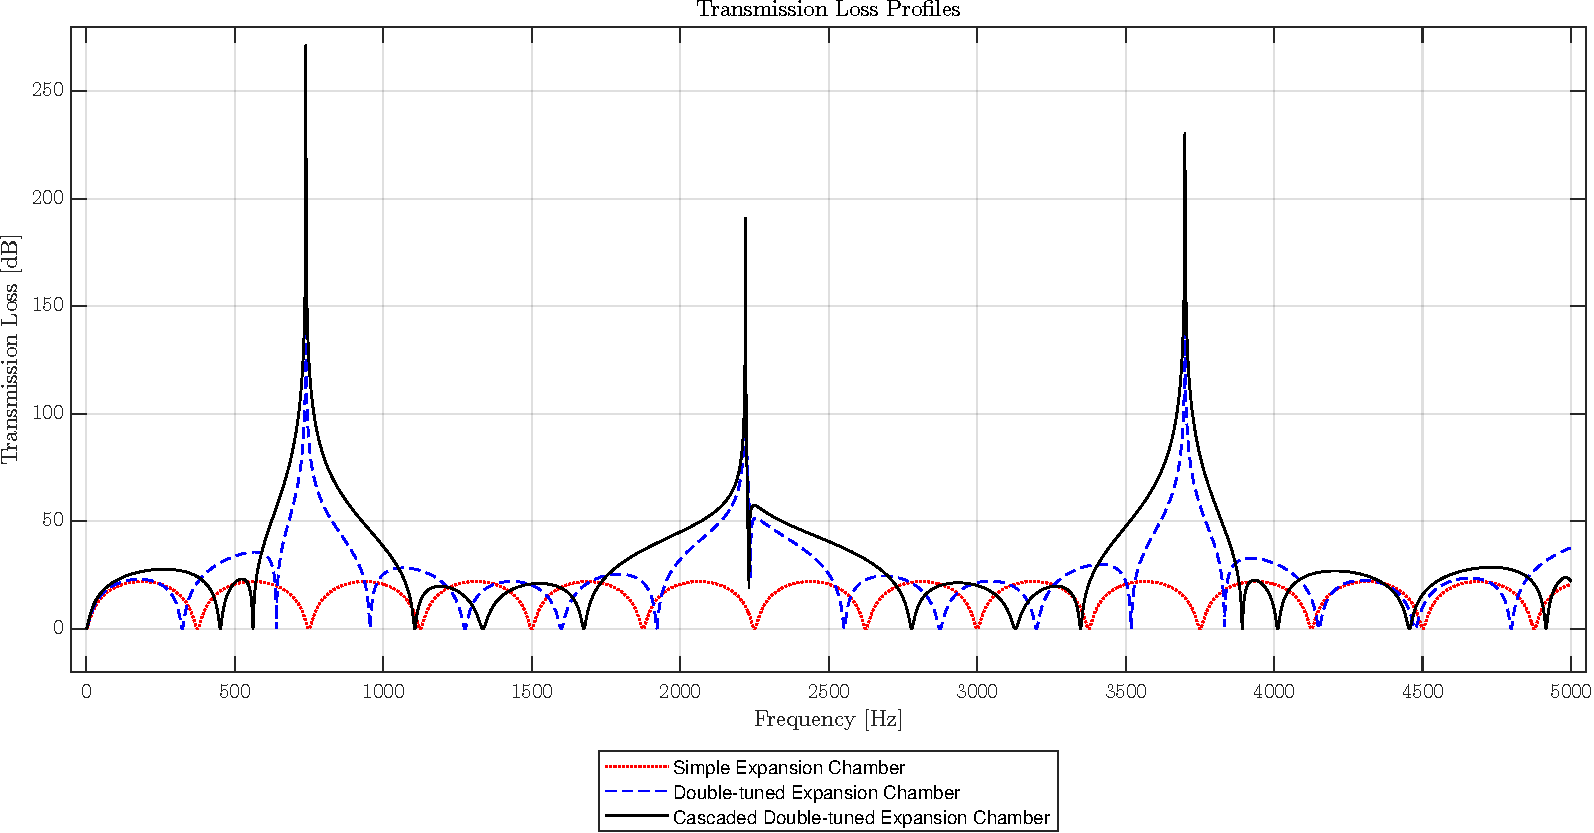
\includegraphics[ scale = 0.675, keepaspectratio ]{Assignment 1 - Question 2 Figure All TL Profiles.pdf}
%
%    \caption{Transmission loss profiles for a simple expansion chamber, a double-tuned expansion chamber, and a cascaded double-tuned expansion chamber muffler.}
%    \label{figure:problem2figure1}
%
%\end{figure}



\subsection*{Problem 2b}

Figure~\ref{figure:problem2figure2} shows the transmission loss profiles for a cascaded double-tuned expansion chamber and a modified version of this muffler.

\vspace{0.25cm}
Two modifications were made to the original muffler:

\begin{enumerate}[itemsep=0.3cm]
  \item The left 3" extension tube in the left chamber was shortened to 2" inches, making the respective muffler section 1" longer.
  \item The left 3" extension tube in the right chamber was lengthened to 4", making the respective muffler section 1" shorter.
\end{enumerate}

%\vspace{0.5cm}
%\begin{figure}[!htb]
%
%    \center
%        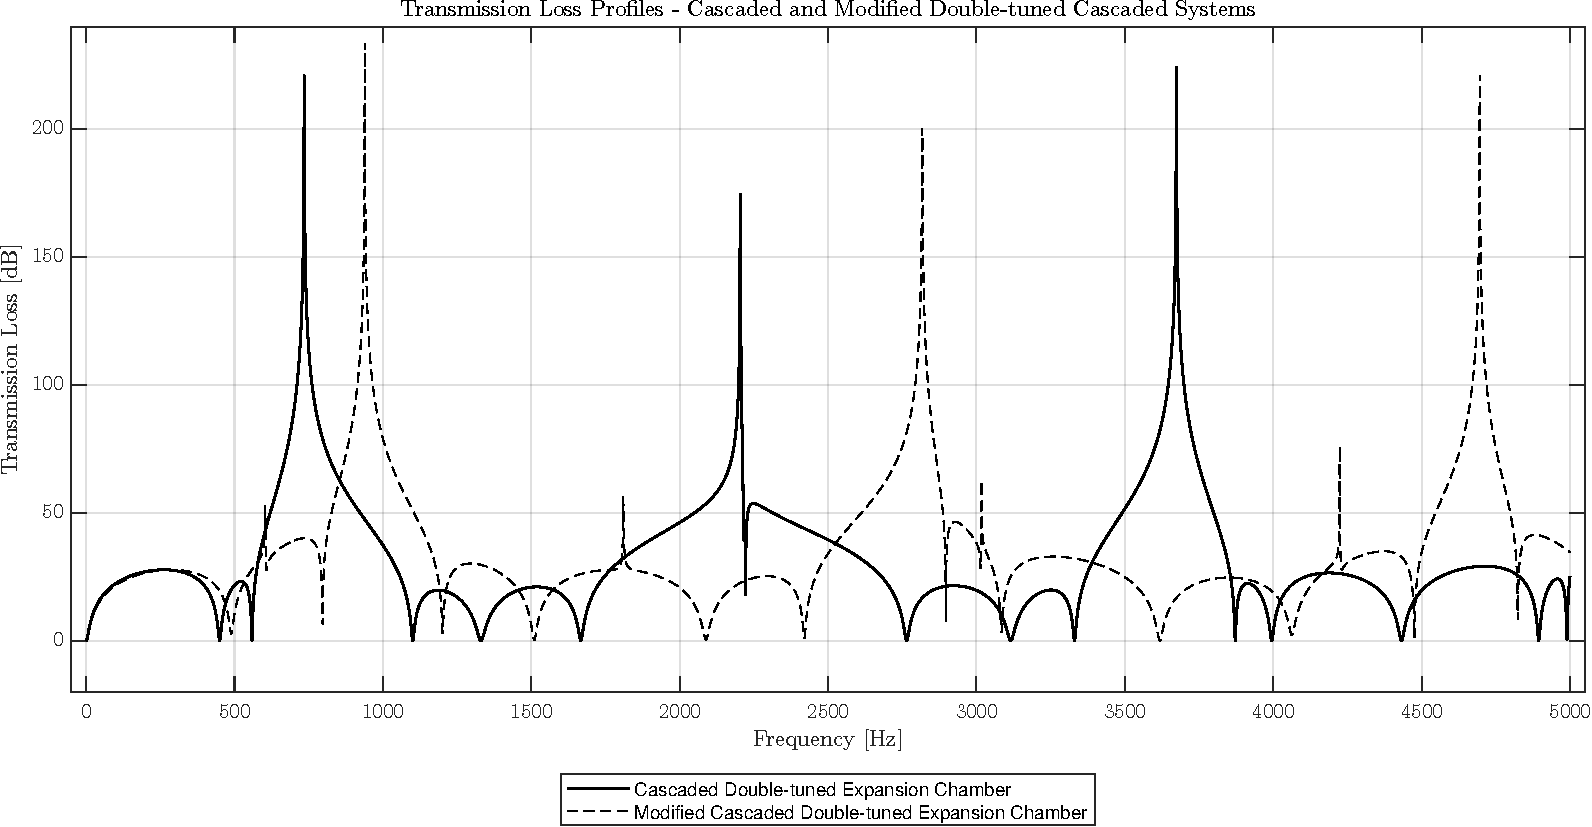
\includegraphics[ scale = 0.675, keepaspectratio ]{Assignment 1 - Question 2 Figure Comparison TL Plot For Cascaded Systems.pdf}
%
%    \caption{Transmission loss profiles for a cascaded double-tuned expansion chamber muffler and a modified version of this muffler.}
%    \label{figure:problem2figure2}
%
%\end{figure}

\vspace{0.25cm}
These modifications change the symmetry of the cascaded system, and allow the resonate frequencies to be changed independently.












\newpage
\section*{Problem 3 - Transmission Loss Measurement}


\vspace{-0.25cm}
The Matlab code for this problem is listed in Appendix~\ref{appendix:problem3}.

\vspace{0.25cm}
Table~\ref{table:mouthpieceAndPip} lists the length of the pipe section and the mouthpiece.

\setlength{\abovecaptionskip}{0pt}
\vspace{0.1cm}
{\renewcommand{\arraystretch}{1.5}
\begin{table}[h!]
    \begin{center}
        \small
        \begin{tabular}{ | c | c | }
            \hline
            \textbf{Item}  &  \textbf{Length [mm]}  \\
            \hline
                Pipe  &  145  \\
                \hline
                \rowcolor{Gray}
                Mouthpiece  &  90  \\
            \hline
        \end{tabular}
    \end{center}
    \caption{Calculated length of the pipe and length of the mouthpiece.}
    \label{table:mouthpieceAndPip}
\end{table}


%\vspace{-0.25cm}
%\subsection*{Problem 3b}
%
%Table~\ref{table:holePlacementSummary} summarizes the placement of the holes for each note relative to the end of the pipe.
%
%\setlength{\abovecaptionskip}{0pt}
%\vspace{0.1cm}
%{\renewcommand{\arraystretch}{1.5}
%\begin{table}[h!]
%    \begin{center}
%        \small
%        \begin{tabular}{ | c | c | c | }
%            \hline
%            \textbf{Note}  &  \textbf{Frequency [Hz]}  &  \textbf{Length from End of Pipe [mm]}  \\
%            \hline
%                C5  &  523      &  n/a  \\
%                \rowcolor{Gray}
%                F5  &  698      &  87.75  \\
%                A5  &  880      &  138.25  \\
%                \rowcolor{Gray}
%                C6  &  1,046    &  0.168  \\
%            \hline
%        \end{tabular}
%    \end{center}
%    \caption{Hole placement distances.}
%    \label{table:holePlacementSummary}
%\end{table}


%\vspace{0.25cm}
%Figure~\ref{figure:bugleRecorderNoteSpectrums} shows the respective spectrum for each of the bugle recorder notes.
%
%\vspace{0.25cm}
%\begin{figure}[!htb]
%    \center
%        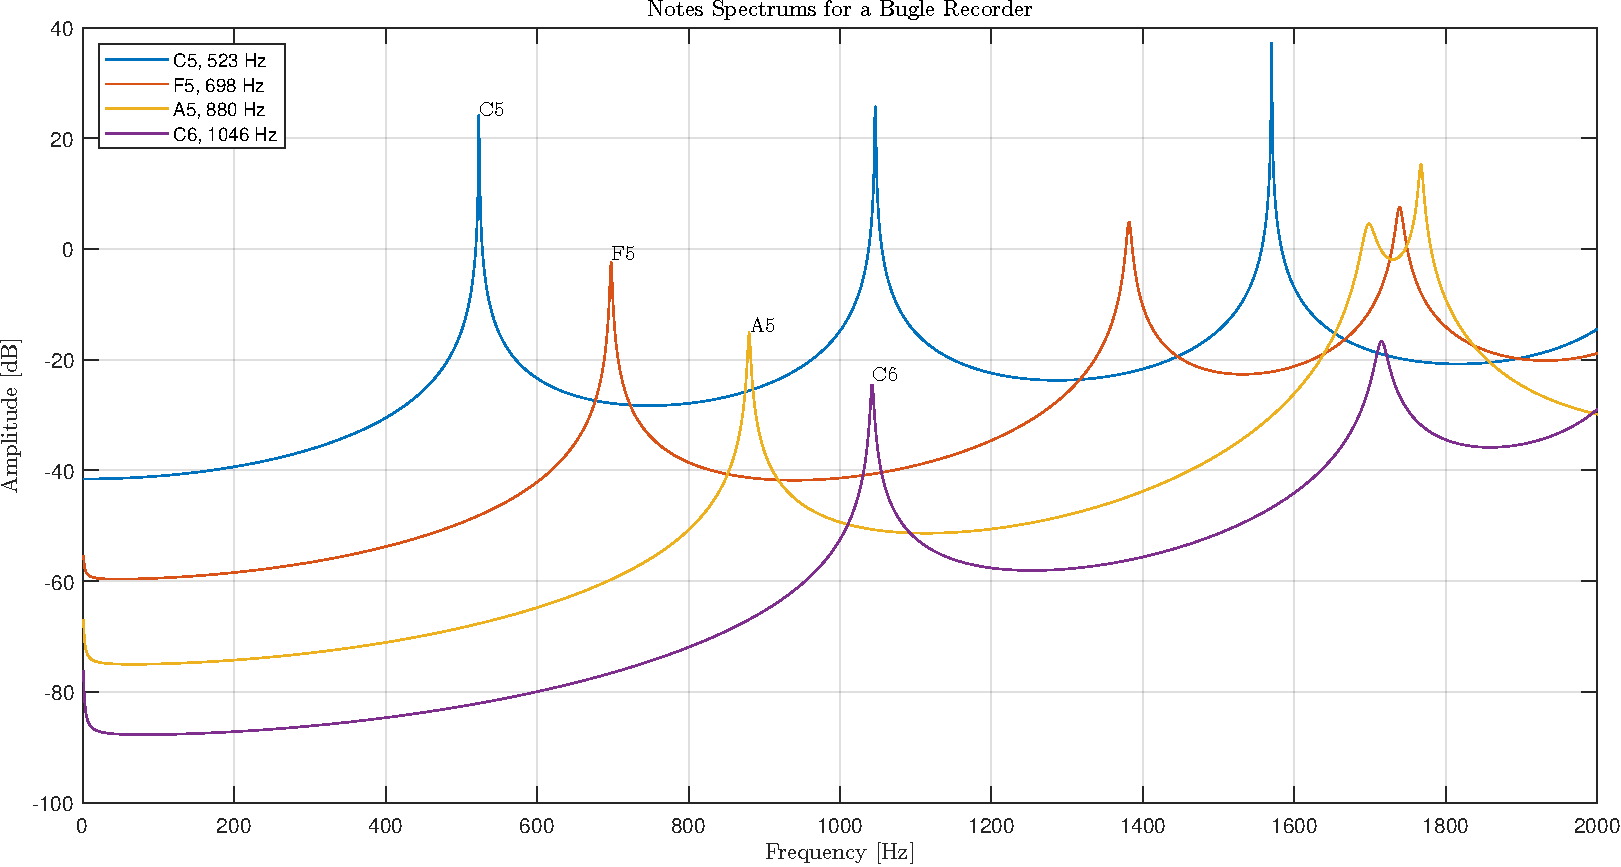
\includegraphics[ scale = 0.6, keepaspectratio ]{Assignment 1 - Question 3 Bugle Recorder Note Spectrums.pdf}
%    \caption{Spectrum for the C5, F5, A5, and C6 bugle recorder notes.}
%    \label{figure:bugleRecorderNoteSpectrums}
%\end{figure}












\newpage
\section*{Problem 4 - Panel Transmission Loss}

The Matlab code for this problem is listed in Appendix~\ref{appendix:problem4}.

\subsection*{Problem 4a}

Table~\ref{table:machNumbers} lists the Mach numbers for each pipe section.  The flow rate is 0.017462 $\frac{m^3}{s}$.

\setlength{\abovecaptionskip}{0pt}
\vspace{0.1cm}
{\renewcommand{\arraystretch}{1.5}
\begin{table}[h!]
    \begin{center}
        \small
        \begin{tabular}{ | c | c | c | }
            \hline
            \textbf{Pipe}  &  \textbf{Area [}{$\mathbf m^2$}\textbf{]}  &  \textbf{Mach Number [unitless]}  \\
            \hline
                Inlet  &  0.000507  &  -0.10047  \\
                \hline
                \rowcolor{Gray}
                Outlet  &  0.00811  &  -0.0062795  \\
            \hline
        \end{tabular}
    \end{center}
    \caption{Calculated Mach numbers.}
    \label{table:machNumbers}
\end{table}



\subsection*{Problem 4b}

\vspace{0.25cm}
Figure~\ref{figure:intakeSystem} shows the transmission loss profiles.

%\vspace{0.25cm}
%\begin{figure}[!htb]
%    \center
%        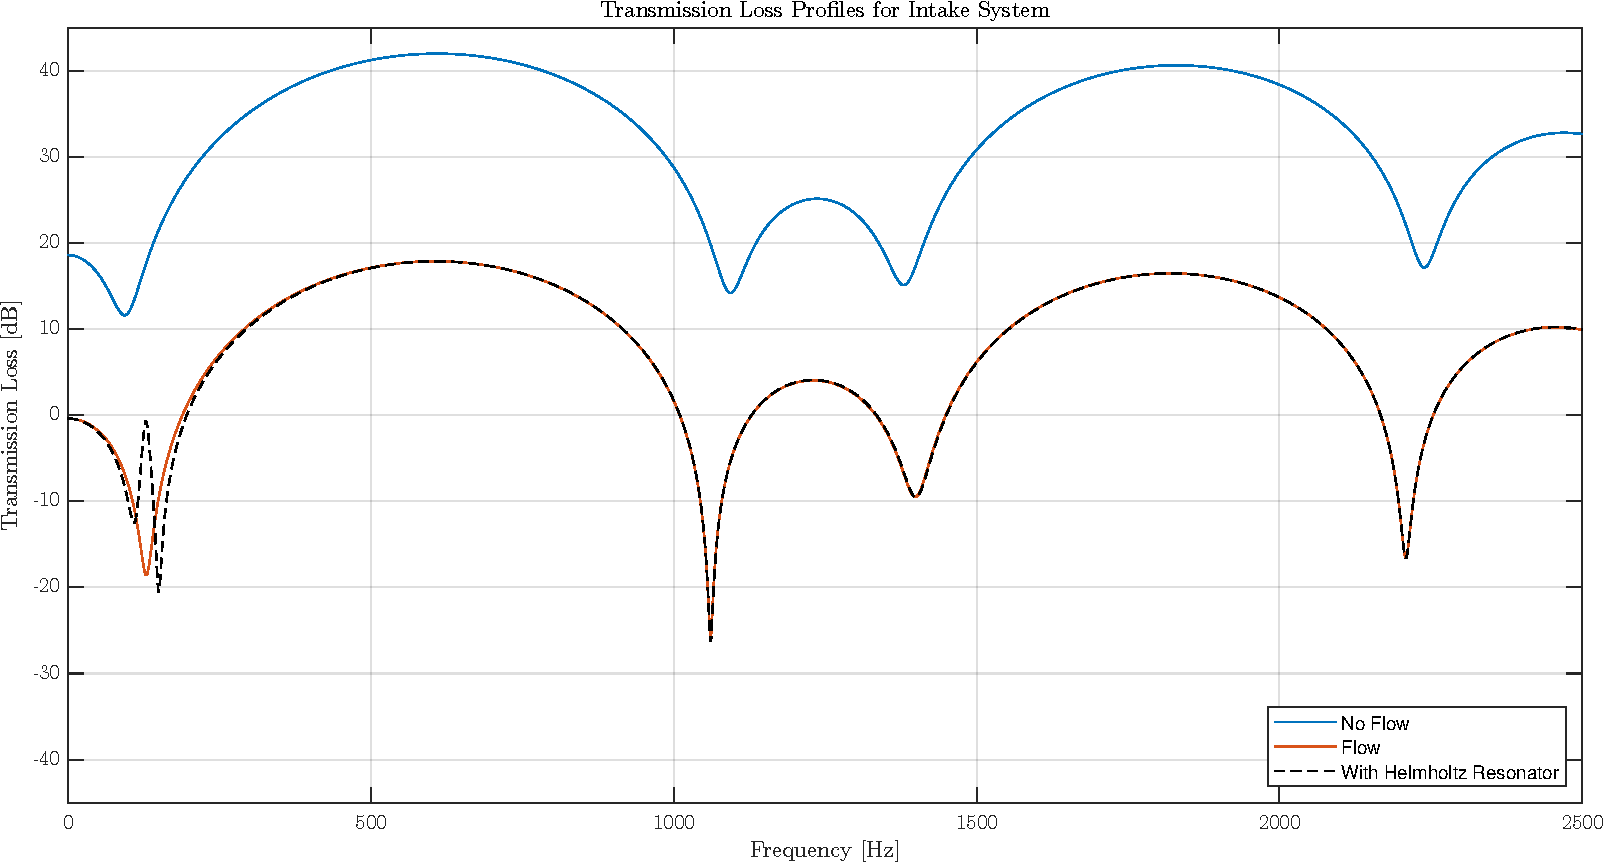
\includegraphics[ scale = 0.6, keepaspectratio ]{Intake System.pdf}
%    \caption{Transmission loss profiles for no flow, flow, and flow with a lossy Helmholtz resonator.}
%    \label{figure:intakeSystem}
%\end{figure}

\vspace{0.25cm}
The addition of flow to the intake system introduces a slight phase delay, a lower overall level of loss (approximately 22 dB), and greater loss at the dips.  The phase delay is easier to see at respective dips in the loss profile.



\vspace{0.25cm}
\subsubsection*{i - Critical Frequency and Coincidence Frequency at 75$^\circ$}

ph



\vspace{0.25cm}
\subsubsection*{ii - Transmission Loss at Angle of Incidence of 75$^\circ$}

ph



\vspace{0.25cm}
\subsubsection*{iii - Transmission Loss for Angles of Incidence between 0-90$^\circ$}

ph



\vspace{0.25cm}
\subsubsection*{iv - Diffuse Transmission Loss}

ph



\newpage
\subsection*{Problem 4c}



\subsection*{Problem 4d}

\vspace{0.25cm}
\subsubsection*{i - Critical Frequency and Coincidence Frequency at 75$^\circ$}

ph

\vspace{0.25cm}
\subsubsection*{ii - Transmission Loss at Angle of Incidence of 75$^\circ$}

ph

vspace{0.25cm}
\subsubsection*{iii - Transmission Loss for Angles of Incidence between 0-90$^\circ$}

ph

\vspace{0.25cm}
\subsubsection*{iv - Diffuse Transmission Loss}





%\vspace{0.25cm}
%Figure~\ref{figure:intakeSystem} shows the transmission loss profiles.


%\newpage
%Table~\ref{table:helmholzResonator} lists the dimensions of the lossy Helmholtz resonator for the 129 Hz notch.
%
%\setlength{\abovecaptionskip}{0pt}
%\vspace{0.1cm}
%{\renewcommand{\arraystretch}{1.5}
%\begin{table}[h!]
%    \begin{center}
%        \small
%        \begin{tabular}{ | l | c | }
%            \hline
%            \textbf{Item}  &  \textbf{Measure]}  \\
%            \hline
%                Cavity Diameter                 &  0.254 m  \\
%                \hline
%                \rowcolor{Gray}
%                Neck Diameter                   &  0.0254 m  \\
%                \hline
%                Neck Length                     &  0.127 m  \\
%                \hline
%                \rowcolor{Gray}
%                Neck Area                       &  0.5e-3 $m^2$  \\
%                \hline
%                Length Correction 1, $L_{o1}$   &  0.711 m  \\
%                \hline
%                \rowcolor{Gray}
%                Length Correction 2, $L_{o2}$   &  0.3 m  \\
%                \hline
%                Cavity Volume                   &  8.0e-5 $m^3$  \\
%                \hline
%                \rowcolor{Gray}
%                Q Factor   &  10  \\
%            \hline
%        \end{tabular}
%    \end{center}
%    \caption{Dimensions of the lossy Helmholtz resonator (see slide 15 of Lecture 3 notes).}
%    \label{table:helmholzResonator}
%\end{table}










\newpage
\section*{Problem 5 - Large Enclosure Design}

The Matlab code for this problem is listed in Appendix~\ref{appendix:problem5}.

\vspace{0.25cm}
ph







\newpage
\section*{Problem 6 - Close-fitting Enclosure Design}

The Matlab code for this problem is listed in Appendix~\ref{appendix:problem5}.

\vspace{0.25cm}
ph






%\newpage
%\section{Appendix - Matlab Code for Problem 1}
%\label{appendix:problem1}
%
%\lstinputlisting[style=Matlab-Pyglike, basicstyle=\fontfamily{pcr}, numbers=left, keepspaces, mlshowsectionrules, basicstyle=\scriptsize]{../ACS_597_Module_1_Question_1_Monday_January_13_2025.m}



%\newpage
%\section{Appendix - Matlab Code for Problem 2}
%\label{appendix:problem2}
%
%\lstinputlisting[style=Matlab-Pyglike, basicstyle=\fontfamily{pcr}, numbers=left, keepspaces, mlshowsectionrules, basicstyle=\scriptsize]{../ACS_547_Module_1_Question_2_Monday_January_27_2025.m}



%\newpage
%\section{Appendix - Matlab Code for Problem 3}
%\label{appendix:problem3}
%
%\lstinputlisting[style=Matlab-Pyglike, basicstyle=\fontfamily{pcr}, numbers=left, keepspaces, mlshowsectionrules, basicstyle=\scriptsize]{../ACS_547_Module_1_Question_3_Wednesday_January_29_2025.m}



%\newpage
%\section{Appendix - Matlab Code for Problem 4}
%\label{appendix:problem4}
%
%\lstinputlisting[style=Matlab-Pyglike, basicstyle=\fontfamily{pcr}, numbers=left, keepspaces, mlshowsectionrules, basicstyle=\scriptsize]{../ACS_547_Module_1_Question_4_Wednesday_January_29_2025.m}



%\newpage
%\section{Appendix - Matlab Code for Problem 5}
%\label{appendix:problem5}
%
%\lstinputlisting[style=Matlab-Pyglike, basicstyle=\fontfamily{pcr}, numbers=left, keepspaces, mlshowsectionrules, basicstyle=\scriptsize]{../ACS_547_Module_1_Question_5_Friday_January_31_2025.m}







\end{document}






% Reference(s):

% https://tex.stackexchange.com/questions/180222/how-to-change-font-size-for-specific-lstlisting


































